\chapter{Introducción}

En este capítulo no deben faltar los siguientes apartados:

\section{Motivación del proyecto}

{Aumento del consumo energético}
En los últimos años ha aumentado el consumo energético en España, en 2014 la demanda 

\begin{figure}[h]
	\centering
	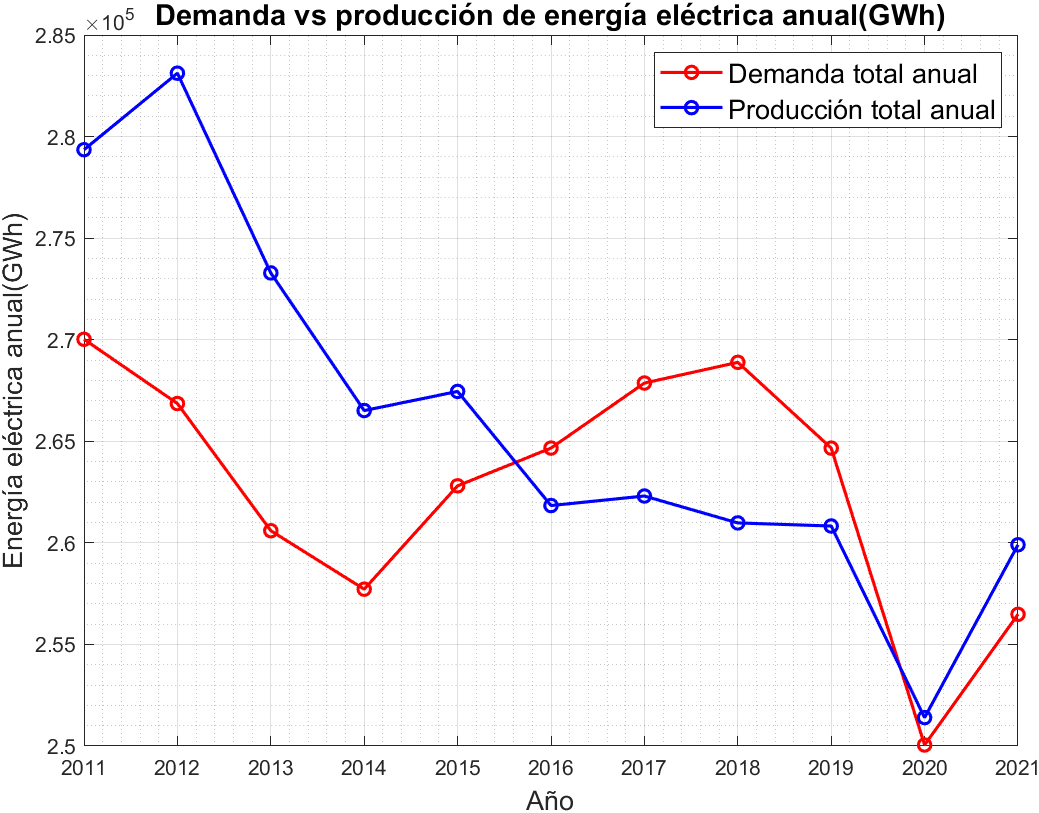
\includegraphics[width=10cm, height=7cm]{figuras/ProdcVSdemAnual}
	\caption[Producción vs demanda de energía eléctrica anual]{Producción vs demanda de energía eléctrica anual. \textit{Fuente: red eléctrica de España} }
	\label{fig:prodcvsdemanual}
\end{figure}



Objetivos del desarrollo sostenible

{Aprovechamiento de energía}
% Aquí irá el gran cantidad de energía que se desperdicia en las fábricas, refinerías, etc.
% Así como se puede aprovechar mediante la termo-fotovoltaíca.



\section{Objetivos}
El objetivo de este estudio es diseñar y simular pilares de dimensiones nanométricas para el aprovechamiento del efecto de campo cercano en un convertidor termo-fotovoltaico, así como determinar la viabilidad de este sistema. 
\begin{itemize}
	\item Modelar un nano-espaciador dentro de los rangos permitidos de los parámetros de los programas de simulación y modelado 3D.
	\item Modelar el emisor y la célula del sistema TPV para que los gradientes térmicos por conducción no lleguen a los bordes.
	\item Simular la transferencia de calor por conducción a través de un nano-espaciador de $SiO_2$ de un sistema TPV para diferentes alturas del nano-espaciador, diferentes materiales de emisor y diferentes resistencias de contacto entre emisor y el nano-espaciador.
	\item Simular la transferencia de calor radiada entre el emisor y la célula para diferentes materiales del emisor y para varias distancias de separación, teniendo en cuenta los efectos de campo cercano en la radiación.
	\item Determinar entre los casos estudiados cuales pueden dar lugar a sistemas de TPV de campo cercano viables.
\end{itemize}


\section{Estructura del documento}

A continuación y para facilitar la lectura del documento, se detalla el contenido de cada capítulo.

\begin{itemize}
\item En el \textbf{capítulo 1} se realiza una introducción del trabajo con la respectiva motivación y objetivos.
\item En el \textbf{capítulo 2} se desarrolla el estado de arte, definiendo los apartados más importantes y resaltando las investigaciones con mayor relevancia.
\item En el \textbf{capítulo 3} se exponen las herramientas y materiales utilizados, así como los criterios de selección.
\item En el \textbf{capítulo 4} se mencionan los métodos seguidos y los cálculos realizados para el desarrollo del trabajo.
\item En el \textbf{capítulo 5} se exponen los resultados obtenidos de las simulaciones.
\item En el \textbf{capítulo 6} se desarrolla la conclusión y se realiza planteamientos para futuros trabajos.
\end{itemize}
